\documentclass{fhnwreport/fhnwreport}

\usepackage{lipsum}
\usepackage[ngerman]{babel}
\usepackage{tikz}
\usetikzlibrary{arrows}
\usetikzlibrary{patterns}
\usetikzlibrary{plotmarks}
%\pgfplotsset{try min ticks=3}
\usepackage{pgfplots}
\pgfplotsset{compat=newest}
\pgfplotsset{max space between ticks=80pt}
\pgfplotsset{max space between ticks=80pt}
\pgfplotsset{
    tick label style={font=\small},
    label style={font=\small},
    legend style={font=\footnotesize}
}
\usepackage[T1]{fontenc}
%\usepackage{textcomp}
%\usepackage[utf8x]{inputenc}
\usepackage[utf8]{inputenc}
\usepackage{amsmath}
\usepackage{amsfonts}
%\usepackage{MnSymbol}
\usepackage{wasysym}
\usepackage{lmodern}   %Type1-Schriftart f\"ur nicht-englische Texte
\usepackage{datetime}
\usepackage{cite}
\usepackage{lipsum}
\usepackage{booktabs}
\usepackage{pdflscape}
\usepackage{longtable}
\usepackage[figuresright]{rotating} % for single-sided printing
\usepackage{xcolor}
\usepackage{colortbl}
\usepackage{hyperref}
\usepackage[titletoc,title]{appendix}
\usepackage{graphicx}
\usepackage{pdfpages}
\usepackage{enumitem}
\usepackage{caption}
\usepackage{gensymb}
\usepackage{pbox}
%\usepackage{draftwatermark}
%\usepackage[nostamp]{draftwatermark}
\usepackage[textsize=footnotesize, textwidth = 17mm, german, colorinlistoftodos]{todonotes}
\usepackage[separate-uncertainty = true]{siunitx}
\usepackage{mathtools}
\usepackage{matlab-prettifier}
\usepackage{spreadtab}
\usepackage{transparent}
\usepackage{relsize}
\usepackage{svg}
\usepackage{multirow}
\usepackage{csquotes}
\usepackage{wrapfig}
%\usepackage[style=mla,backend=bibtex]{biblatex}
%\addbibresource{bibliography/bibliography.bib}

\definecolor{dkgreen}{rgb}{0,0.6,0}
\definecolor{gray}{rgb}{0.5,0.5,0.5}
\definecolor{mauve}{rgb}{0.58,0,0.82}

\lstdefinestyle{java}{
    language            = Java,
    aboveskip           = 3mm,
    belowskip           = 3mm,
    showstringspaces    = false,
    columns             = flexible,
    basicstyle          = {\scriptsize\ttfamily},
    numbers             = left,
    numberstyle         = \tiny\color{gray},
    keywordstyle        = \color{blue},
    commentstyle        = \color{dkgreen},
    stringstyle         = \color{mauve},
    breaklines          = true,
    breakatwhitespace   = true,
    tabsize             = 3
}
\lstdefinestyle{Matlab-editor-2}{%
  style               = MatlabBaseStyle@mlpr,
  mllastelementstyle  = \color{black}                    ,
  mlkeywordstyle      = \color[RGB]{000,000,255}         ,
  mlcommentstyle      = \color[RGB]{034,139,034}         ,
  mlstringstyle       = \color[RGB]{160,032,240}         ,
  mlsyscomstyle       = \color[RGB]{178,140,000}         ,
  mlsectiontitlestyle = \commentStyle@mlpr      \bfseries,
  mlsharedvarstyle    = \color[RGB]{000,163,163}         ,
  mlplaceholderstyle  = \mleditorphstyle,
  basicstyle          = \ttfamily\scriptsize,
  numbers             = left,
}


%\SetWatermarkText{\texttt{Entwurf}}
%\SetWatermarkText{Entwurf}
%\SetWatermarkLightness{0.9}

\setcounter{secnumdepth}{5} % up to and including paragraph. Not working atm.
\setcounter{tocdepth}{2}

\DeclarePairedDelimiter\abs{\lvert}{\rvert}%

%\renewcommand{\thesubsubsection}{\arabic{subsubsection}}

%\renewcommand{\thefootnote}{\roman{footnote}}
\renewcommand{\thefootnote}{\Roman{footnote}}

\hypersetup{%
  bookmarksnumbered = true,
  colorlinks = true,
  linkcolor  = black,
  citecolor  = black,
  %urlcolor   = blue,
  urlcolor   = black,
  %hidelinks  = false
}

\title{%
    \textbf{\Huge{\texttt{BAT6}}} \\
}

%\newcommand{\colfigure}[3]{%
    \begin{minipage}[c][][b]{0.485\textwidth}
        #1
    \end{minipage}
    \hspace{0.03\textwidth}
    \begin{minipage}[c][][b]{0.485\textwidth}
        {\raggedleft%
            \includegraphics[width=0.9\textwidth]{#2}%
        }
        \captionof{figure}{#3}
    \end{minipage}\\%
}

%\newlist{longenum}{enumerate}{5}
\setlist[longenum,1]{label=\roman*)}
\setlist[longenum,2]{label=\alph*)}
\setlist[longenum,3]{label=\arabic*)}
\setlist[longenum,4]{label=(\roman*)}
\setlist[longenum,5]{label=(\alph*)}

\def\code#1{\texttt{#1}}

\DeclareSIUnit[number-unit-product = {}]
    \partspermillion{ppm}
\DeclareSIUnit[number-unit-product = {}]
    \permille{\perthousand}



\begin{document}

\begin{titlepage}

    \maketitle
    \vspace{40mm}
    \begin{center}
        \Large{Solar Panel Emulator}%
    \end{center}

    \vspace{50mm}
    %\vspace{90mm}

    %\hspace{-20mm}
    \begin{tabular}{r|l}

        \textsc{\textbf{Degree Program}}
        & EIT\\
        [4mm]

        \textsc{\textbf{Module}}
        & Projekt 3 \\
        [4mm]

        \textsc{\textbf{Team}}
        & 2 \\
        [4mm]

        \textsc{\textbf{Sponsor}}
        & Hanspeter Gysin \\
        [4mm]

        \textsc{\textbf{Coaches}}
        & Hanspeter Gysin, Peter Ganzmann, Matthias Meier,\\
        & Anita Gertiser, Bonnie Domenghino\\
        [4mm]

        %\textsc{\textbf{A}}
        %& Reto Freivogel, Alexander Murray, Raphael Frey\\
        %[4mm]

        \textsc{\textbf{Version}}
        & \code{1} \\
    \end{tabular}
    %\end{center}

\end{titlepage}


% **************************************************************************** %
\clearpage
\section*{Abstract}
\label{sec:abstract}
% **************************************************************************** %
% relevance/motivation
% problem statement
% approach: how as the problem solved
% results
% conclusions
% keywords

% introduction
% research problem
% body
% results
% conclution

 % introduction
Simulating  solar  modules  in  a laboratory  environment  currently  requires
expensive  and complex  equipment, hindering  development of  new solar  power
products. To  facilitate  research  into  solar  panel  behavior,  a  low-cost
solution for simulating solar modules is needed.

% approach
This  report details  our  efforts in  developing and  building  a device  for
this  purpose. We  developed a  model  for  describing solar  module  behavior
mathematically, which is  capabable of describing both a single  solar cell as
well  as  configurations  of  multiple  cells. The  hardware  is  based  on  a
microcontroller, responsible  for interacting  with the  outside world,  and a
voltage converter, used  to generate the desired voltages and  currents on the
device's output.

% results
At  this point,  the device  is not  operational. Due to  a design  error, our
circuit  overloads  the  voltage converter,  causing  irreparable  damage. The
likely cause  of this are  overlong connections between the  voltage converter
and other  components.  The  next step  in finalising the  device would  be to
design a new circuit board for fixing this issue.



% **************************************************************************** %
\clearpage
\pagestyle{empty}
{
    \renewcommand{\thispagestyle}[1]{}
    \tableofcontents
    \vspace{30mm}
    \subsection*{Versionsgeschichte}
    \begin{itemize}
        \item[]
            %\emph{20.10.2015:} \texttt{Version 1}
            \emph{\today} \texttt{Version 1}
    \end{itemize}
}

\clearpage
\setcounter{page}{1}
\pagestyle{headings}
% **************************************************************************** %

% **************************************************************************** %
\clearpage
\section{Einleitung}
\label{sec:introduction}
% **************************************************************************** %
% Structured according to Gertiser's feedback:
% 1) Worum geht es?
% 2) Ziel und Anforderungen
% 3) Umsetzung -> Grobkonzept
% 4) Resultate
% 5) Aufbau der Arbeit

% TODO: source for expensive shit

Verifying the correct operation of equipment  used for testing solar arrays is
currently difficult in  a controlled laboratory environment,  as no affordable
solutions for this exist on the open market. To address this issue, the aim of
this project was the development of a device capable of emulating the behavior
of a  photovoltaic module. With this  device, test equipment  for photovoltaic
modules can be verified to function  as specified in a laboratory conveniently
and affordably.

The primary characteristics  of our device should be compactness  (usable in a
standard  laboratory environment),  the  capability to  emulate varying  solar
irradiation levels,  being able  to be  used in  series with  other emulators,
effiency with  regards to  power consumption  and losses,  and to  emulate the
characteristic  curve of  an actual  PV module. A  more detailed  list of  the
technical  requirements  can be  found  in  the specifications  (see  appendix
\code{XXX (link to Lastenheft)}). %TODO

A microcontroller and a constant-current, constant-voltage step-down converter
constitute the core of our device.  The microcontroller performs IO operations
and implements  the regulation loop  used to control the  step-down converter,
whereas  the  step-down converter  generates  the  output voltage  and  output
current  corresponding  to  the  desired  operating  point  from  a  DC  power
supply. The  entire design  is  based  around a  custom  PCB,  enabling us  to
optimise impedances of  connections between critical components. Additionally,
we can get very close in behavior to a potentially mass-produced product since
trace lenghts, routing  and component placement are crucial  (see also section
\ref{sec:verification}, beginning on page \pageref{sec:verification}).

The device has a simple yet powerful user interface which can be controlled by
a push-twist button and a modern OLED display. The device can also be remotely
monitored and controlled from a PC via USB interface and custom software built
on the  Qt application framework  and is  compatible with all  major operating
systems~\cite{ref:qt}.  Our  device can emulate fairly  complex configurations
of cells thanks to an efficient  use of computation resources and its powerful
microprocessor.

Sections  \ref{sec:task}   (p.  \pageref{sec:task}ff)   and  \ref{sec:concept}
(p.   \pageref{sec:concept}ff)   of   this   report   deal   with   the   task
itself  and  the  basic   concept  behind  our  solution. Component  selection
and   PCB  design   are  documented   in  sections   \ref{sec:components}  (p.
\pageref{sec:components}ff)   and   \ref{sec:pcb}   (p.   \pageref{sec:pcb}ff)
respectively, while section \ref{sec:software}  is concerned with the software
(p.  \pageref{sec:software}ff).   Lastly, section  \ref{sec:verification}  (p.
\pageref{sec:verification}ff) deals  with testing  the device  including error
analysis, and the  conclusion can be found in  section \ref{sec:conclusion} on
page \pageref{sec:conclusion}.


% **************************************************************************** %
\clearpage
\section{Aufgabenstellung}
\label{sec:aufgabenstellung}
% **************************************************************************** %
Aufgabenstellung, Basic Info \"uber PV-Module



% **************************************************************************** %
\clearpage
\section{Grundkonzept}
\label{sec:grundkonzept}
% **************************************************************************** %
Grundkonzept der L\"osungsansatzes, allgemeine \"Uberlegungen

Die  Aufgabe  besteht  darin  die   UI-Kennlinie  einer  Solarzelle  durch  eine
elektronische Schaltung k\"unstlich nachbilden zu k\"onnen.

(insert example UI Kennlinie)





% **************************************************************************** %
\clearpage
\section{Komponenten}
\label{sec:components}
% **************************************************************************** %
Es wird  in  Detail  beschrieben,  welche  elektronische Komponenten aus welchem
Grund ausgew\"ahlt worden sind.

% **************************************************************************** %
\subsection{36V Netzteil und Netzeingang}
% **************************************************************************** %

Die  maximale Ausgangsleistung wurde grob berechnet  mit  $\SI{24}{\volt}  \cdot
\SI{3}{\ampere} = \SI{72}{\watt}$.

Da das Aufbauen eines eigenen Netzteils f\"ur die notwendige Ausgangsleistung zu
aufw\"andig und  teuer  gewesen  w\"are,  entschieden wir uns f\"ur ein externes
Netzger\"at  dass  im  Geh\"ause  montiert werden kann. Das verwendete  Netzteil
liefert   \SI{36}{\volt}   und   \SI{75}{\watt}  und  ist   in   der   Abbildung
\ref{fig:circuit:mains-input} als $N_2$ zu sehen.

\begin{figure}[th!]
    \center
    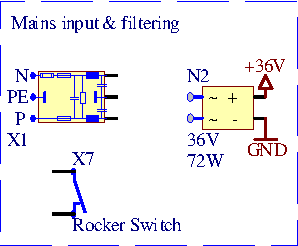
\includegraphics[width=.35\textwidth]{images/circuit/mains-input.pdf}
    \caption{Netzspannung wird gefiltert und auf 36V DC durch ein externes Netzmodul transformiert}
    \label{fig:circuit:mains-input}
\end{figure}

Weiter  wird  eine  Netzeingangs-Steckverbinder  mit integriertem Netzfilter und
Sicherung  verwendet,  was  in der Abbildung  \ref{fig:circuit:mains-input}  als
$X_1$  zu  sehen  ist. Ein auf der R\"uckseit des Geh\"auses montierter Schalter
$X_7$ erlaubt das Ein- und Ausschalten des Endproduktes.



% **************************************************************************** %
\subsection{Spannungsversorgungen}
% **************************************************************************** %

F\"ur die digitale  Logik  werden  die  zwei  Spannungspegel  \SI{5}{\volt}  und
\SI{3.3}{\volt} ben\"otigt.

\begin{figure}[th!]
    \center
    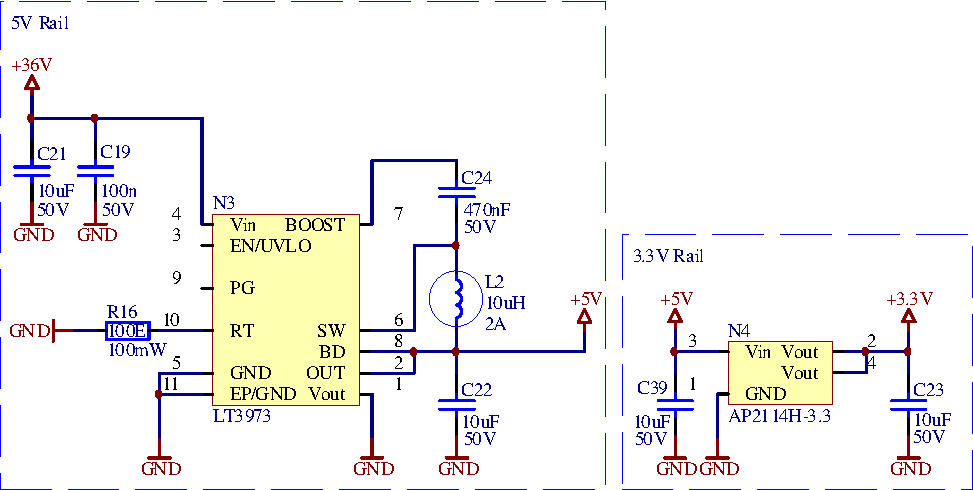
\includegraphics[width=.75\textwidth]{images/circuit/5v-3v-rails.pdf}
    \caption{Speisung f\"ur 5V mittels Abwertswandler (links) und Speisung f\"ur 3.3V mittels Linearregler (rechts)}
    \label{fig:circuit:rails}
\end{figure}

Die  \SI{36}{\volt} vom Netzteil werden mittels eines getakteten  DC-DC-Wandlers
auf \SI{5}{\volt} transformiert,  was  in  der Abbildung \ref{fig:circuit:rails}
vom Bauteil $N_3$ verwirklicht wird.

Die  \SI{5}{\volt}  werden  von  einem  Linearregler  $N_4$ auf  \SI{3.3}{\volt}
gestuft. Ein Linearregler wurde  gew\"ahlt  damit  die  \SI{3.3}{\volt} Speisung
m\"oglichst  St\"orfrei  bleibt  --  Getaktete  Wandler  verursachen  viel  mehr
St\"orung. Somit  wird  verhindert,  dass  die DACs und ADCs verrauscht sind und
ungenau messen.


% **************************************************************************** %
\subsection{LT3741}
% **************************************************************************** %

There are  many reasons why the LT3741 was chosen to regulate the output voltage
of this device. The most important reasons are listed here.
\begin{itemize}
    \item \textbf{Re-inventing the wheel.}
        Switch-mode regulators aren't new technology. They've been studied and perfected
        over decades by many engineers. For  this  reason  we decided against building a
        regulator  descretely  and  instead  opted  to  use  an  existing  regulator  if
        available.
    \item \textbf{Voltage and current requirements.}
        The device is specified to  output  voltage  levels  between  \SI{0}{\volt}  and
        \SI{24}{\volt} and current levels between \SI{0}{\ampere} and \SI{3.5}{\ampere}.
        Further,  the  ripple voltage is specified to be $\le\SI{300}{\milli\volt}$  and
        the ripple current  is  specified to be $\le\SI{100}{\milli\ampere}$. The LT3741
        fulfills all of these requirements.
    \item \textbf{The importance of power absorption.}
        Most switch-mode  regulators  are  only  able  to  \emph{supply}  power, but are
        incapable  of  \emph{absorbing} power. Because our device may  be  connected  in
        series (or parallel) with other power  supplies,  it  must  have  the ability to
        absorb  power  to  (which is the case if, say, it were connected  to  a  voltage
        source   outputting   a   higher  voltage  level  than  our  own).  A  so-called
        \emph{synchronous  converter} possesses this property and the LT3741 is  one  of
        them.
    \item \textbf{Control inputs.}
        The LT3741 was chosen  because  it has dedicated input control pins for directly
        changing  the  regulated  output  current.  This makes the design a lot simpler,
        because no complicated additional circuitry is required.
\end{itemize}

\begin{figure}[th!]
    \center
    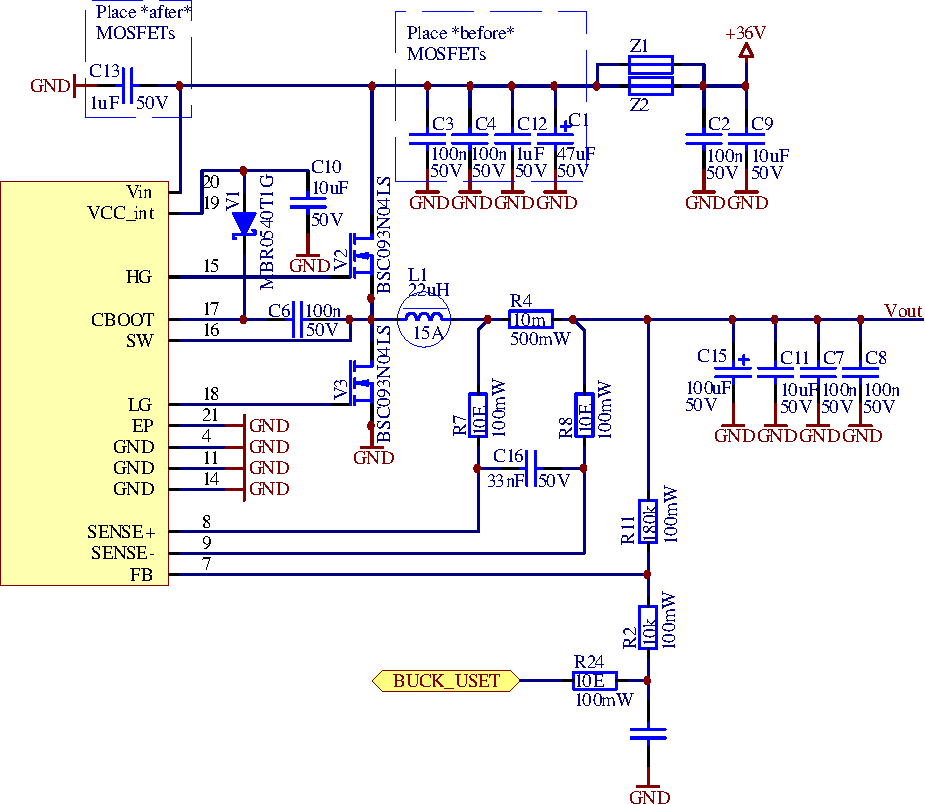
\includegraphics[width=.75\textwidth]{images/circuit/buck.pdf}
    \caption{Herzst\"uck des Projektes: Aufbau des LT3741 CVCC Synchronwandler}
    \label{fig:circuit:buck}
\end{figure}

With the LT3741 selected, the selection of  components  required  to control the
LT3741 are discussed next.

% **************************************************************************** %
\subsubsection{Bypass Capacitors}
% **************************************************************************** %

The LT3741 is powered by the \SI{28}{\volt}  rail, which can be seen in Figure
\ref{fig:circuit:buck} in the  top right. The switching of  the MOSFETs causes
the LT13741  to consume high amounts  of power in short  bursts. This leads to
the LT3741  feeding high  frequency disturbance  back into  the \SI{28}{\volt}
rail, which  could lead  to disturbances  in the  rest of  the circuit  if not
handled correctly.  As a countermeasure,  a multitude of different ceramic and
electrolytic bypass  capacitors in parallel  are used.  Additionally,  we used
ferrite beads, placed  in series with the supply to  absorb any high frequency
feedback.


% **************************************************************************** %
\subsubsection{Switching Frequency}
% **************************************************************************** %

There is a trade-off when  selecting the switching frequency $f_S$. The higher
$f_S$,  the  lower the  output  ripple  voltage  will be. However,  the  power
consumption will also  increase due to switching losses.   Generally, $f_S$ is
to be maximised to reduce ripple.

Because so  much depends  on $f_S$,  it is more  convenient to  determine this
value empirically through simulations. The  most sutiable value was determined
to be $f_S \approx\SI{800}{\kilo\hertz}$. In the remaining calculations, $f_S$
is assumed to be \SI{1}{\mega\hertz} to allow for some leeway.

A specific  resistor on one  of the LT3741's inputs  is used to  configure the
switching frequency $f_S$.


% **************************************************************************** %
\subsubsection{Inductor Selection}
% **************************************************************************** %

The size of the inductor $L_1$, as illustrated in figure \ref{fig:circuit:buck},
was calculated using formula \ref{eq:circuit:buck:inductor}
\begin{equation}
    L_1 = \left( \frac{U_{in} \cdot U_{out} - U_{out}^2}{0.3 \cdot f_S \cdot I_O \cdot U_{in}} \right) = \SI{6}{\micro\henry}
    \label{eq:circuit:buck:inductor}
\end{equation}
where $U_{in}$ is the  input  voltage  \SI{28}{\volt},  $U_{out}$  is the output
voltage at peak power (which exists at $U_{out} = \SI{14}{\volt}$), $f_S$ is the
switching frequency \SI{1}{\mega\hertz} and $I_o$ is the maximum output current,
assumed   to   be   $I_o  =  \SI{5}{\ampere}$  for   some   additional   leeway.

We ended up selecting a  larger  inductor  of  $L_1  = \SI{22}{\micro\henry}$ to
further decrease ripple current.

In addition to the value of  the  inductor, the maximum current rating, DCR, and
saturation  current are also important factors to consider. The maximum  current
of the inductor is calculated using formula 
\ref{eq:circuit:buck:inductor_peak}
\begin{equation}
    I_{L_{1_{peak}}} = I_O + \left( \frac{U_{in} \cdot U_{out} - U_{out}^2}{2 \cdot f_S \cdot L_1 \cdot U_{in}} \right) = \SI{5.2}{\ampere}
    \label{eq:circuit:buck:inductor_peak}
\end{equation}
Where $L$  is  the  value  of  the selected inductor, \SI{22}{\micro\henry}. The
saturation  current  of the inductor was sized factor $1.2$ higher than the peak
current.
\begin{equation}
    I_{L_{1_{saturation}}} = 1.2 \cdot I_{L_{1_{peak}}}
    \label{eq:circuit:buck:inductor_saturation}
\end{equation}

A  list  of  candidates  matching  the  above  parameters  are  listed in  table
\ref{tab:circuit:buck:inductor}.

\begin{table}[th!]
    \begin{center}
        \caption{}
        \label{tab:circuit:buck:inductor}
        \begin{tabular}{lcccc}
            \toprule
            Digikey         & Price (CHF) & Inductance (\SI{}{\micro\henry}) & DCR (\SI{}{\ohm}) & Ohmic Loss (\SI{}{\watt}) \\
            \midrule
            \rowcolor{lightgray}
            732-4237-1-ND   & 8.03        & 22                               & 0.007             & 0.175  \\
            732-2179-1-ND   & 6.4         & 47                               & 0.0335            & 0.8375 \\
            732-2177-1-ND   & 6.4         & 22                               & 0.0146            & 0.365  \\
            \bottomrule
        \end{tabular}
    \end{center}
\end{table}

It  is  clear that the one with the lowest DCR will be the most optimal. The one
highlighted in grey is the one we chose.



% **************************************************************************** %
\subsubsection{MOSFET selection}
% **************************************************************************** %

Die  Bauteile  $V_1$  und  $C_6$  bilden  zusammen  mit  dem  MOSFET  $V_2$  ein
High-Side-Schalter. Im Gegensatz zu einem nicht-synchronen Schaltregler befindet
sich  an  der Stelle wo normalerweise eine Freilaufdiode sein sollte ein zweiter
MOSFET $V_3$. Dieser erm\"oglicht  eine  Spannungsregelung in der gegengesetzten
Richtung -- sprich, sie erm\"oglicht eine Leistungsaufnahme, was, wie oben schon
erw\"ant wurde, kritisch ist.

Bei  der  Auswahl von passenden MOSFETs sind die  Parameter  $Q_G$  (Total  Gate
Charge),  $R_{DS_{(on)}}$  (On-Resistance),  $Q_{GD}$  (Gate to  Drain  Charge),
$Q_{GS}$ (Gate to Source  Charge),  $R_G$  (Gate Resistance), sowie $U_{GS}$ und
$U_{DS}$, $I_{D_{max}}$ und $U_{GS_{THR}}$ kritische Parameter.

Der  maximale  Drain-Strom  kann mit der Formel  \ref{eq:circuit:buck:mosfet_id}
berechnet werden

\begin{equation}
    I_{D_{max}} = I_O + \left( \frac{U_{in} \cdot U_{out} - U_{out}^2}{2 \cdot f_S \cdot L \cdot U_{in}} \right) = \SI{5.2}{\ampere}
    \label{eq:circuit:buck:mosfet_id}
\end{equation}

wobei $I_O$ der maximale Ausgangsstrom  von  \SI{5}{\ampere}  ist,  $U_{in}$ die
Eingangsspannung von  \SI{36}{\volt}  ist,  $U_{out}$  die  Ausgangsspannung bei
gr\"osster  Leistung  ist   (\SI{18}{\volt}),   $f_S$   die  Schaltfrequenz  von
\SI{1}{\mega\hertz}  ist  und  $L$  die  Spule  von  \SI{22}{\micro\henry}  ist.

$U_{DS}$   wurde   h\"oher  gew\"ahlt  als  die  Eingangsspannung:   $U_{DS}   >
\SI{36}{\volt}$.

Der LT3741 liefert als maximale Gate-Steuer-Spannung $U_{GS}$  \SI{5}{\volt}. Da
der LT3741 w\"ahrend dem Aufstartvorgang Steuersignale knapp unter \SI{3}{\volt}
liefert,   muss   die   Gate-Threshold-Spannung   $U_{GS_{THR}}$   kleiner   als
\SI{2}{\volt} gew\"ahlt werden. $U_{GS_{min}}$ muss gr\"osser  als \SI{5}{\volt}
sein.

Leistungsverluste der MOSFETs sind einerseits verbunden mit ohmsche  Verluste --
abh\"angig  von  $R_{DS_{(on)}}$  --  sowie   verbunden  mit  Schaltverluste  --
abh\"angig von $Q_{GS}$ und $Q_{GD}$.

Der    Leistungsverlust    im    High-Side   MOSFET   kann   mit   der    Formel
\ref{eq:circuit:buck:mosfet_ploss} approximiert werden

\begin{multline}
    P_{LOSS} = (\textrm{ohmic loss}) + (\textrm{transission loss}) \\
             \approx \left( I_O^2 \cdot R_{DS_{(on)}} \cdot \rho_T \right)
                    + \left( \frac{U_{in} \cdot I_O}{\SI{5}{\volt}} \cdot \left(Q_{GD} + Q_{GS} \right) \cdot \left( 2 \cdot R_G + R_{PU} + R_{PD} \right) \cdot f_S \right) \\
    \label{eq:circuit:buck:mosfet_ploss}
\end{multline}

wobei $\rho_T$ ein temperaturabh\"angiger Parameter vom Einschaltwiderstand ist.
Bei \SI{70}{\celsius} betr\"agt $\rho_T \approx 1.3$. $R_{PD}$ und $R_{PU}$ sind
die  Ausgangsimpedanzen  vom  LT3741  und  betragen  \SI{1.3}{\ohm}   respektive
\SI{2.4}{\ohm}.

Der  Low-Side MOSFET sollte einen m\"oglichst kleinen $R_{DS_{(on)}}$ haben  und
ein    Total-Gate-Charge    $Q_C    \leq    \SI{30}{\nano\coulomb}$    besitzen.

Ein  weiterer Verlust sind die Schaltverl\"uste der internen  MOSFET-Treiber  im
LT3741. Die Total Gate Charge $Q_C$ muss  w\"ahrend  jedem  Zyklus  geladen  und
wieder   entladen   werden.   Diese   Verl\"uste   k\"onnen   mit   der   Formel
\ref{eq:circuit:buck:switching_loss} berechnet werden,

\begin{equation}
    P_{LOSS\_LDO} \approx \left( (U_{in} - \SI{5}{\volt} \right) \cdot \left( Q_{GLG} + Q_{GHG} \right) \cdot f_S
    \label{eq:circuit:buck:switching_loss}
\end{equation}

wobei $G_{GLG}$ die  Low-Side  Gate-Charge $G_C$ ist und $G_{GHG}$ die High-Side
Gate-Charge ist.

In  der  Tabelle  \ref{tab:circuit:buck:mosfet}  sind  verschiedene MOSFET-typen
aufgelistet, die in den oben genannten Parametern passen. Dabei wurde $P_{LOSS}$
und $P_{LOSS\_LDO}$ f\"ur jeden Kandidaten berechnet.

\begin{table}[th!]
    \begin{center}
        \caption{}
        \label{tab:circuit:buck:mosfet}
        \begin{tabular}{cccccccccc}
            \toprule
            $R_{DS_{(on)}}$ & $Q_{GD}$ & $Q_{GS}$ & $R_G$ & $U_{GS_{THR}}$ & Ohmic Loss & Transision Loss & Total Loss & Drive Loss \\
            \midrule
            0.0032          & 4        & 2.5      & 0.4   & 2.5            & 0.104      & 1.0296          & 1.1336     & 0.806 \\
            0.0039          & 7        & 9        & 2.4   & 3.3            & 0.12675    & 4.8384          & 4.96515    & 1.984 \\
            0.0042          & 7        & 9        & 2.4   & 3.3            & 0.1365     & 4.8384          & 4.9749     & 1.984 \\
            0.008           & 2        & 4.5      & 3     & 2              & 0.26       & 2.2464          & 2.5064     & 0.558 \\
            0.0067          & 5.3      & 3.9      & 1.5   & 1              & 0.21775    & 2.18592         & 2.40367    & 0.7998 \\
            \rowcolor{lightgray}
            0.0093          & 2        & 4.9      & 1     & 2              & 0.30225    & 1.39104         & 1.69329    & 1.488 \\
            0.019           & 8        & 4        & 1.3   & 2              & 0.6175     & 2.6784          & 3.2959     & 1.798 \\
            0.0095          & 7.5      & 6        & 1     & 3              & 0.30875    & 2.7216          & 3.03035    & 1.736 \\
            \bottomrule
        \end{tabular}
    \end{center}
\end{table}

Vergleicht  man  \emph{Total  Loss}  und  \emph{Drive Loss}, w\"ahre der oberste
MOSFET  geeigneter. Aus Kostengr\"unden und  generell  schlechter  Dokumentation
wurde  aber  der   n\"achst  bessere  MOSFET  gew\"ahlt  --  hier  mit  hellgrau
hervorgehoben.

Es  wird  f\"ur  den  High-Side  MOSFET wie auch f\"ur den Low-Side  MOSFET  der
gleiche Typ verwendet.



% **************************************************************************** %
\subsubsection{Measurement of Output Voltage and Output Current}
% **************************************************************************** %

Der  LT3741  ist  sowohl   Spannungsgesteuert   wie   auch  Stromgesteuert.  Der
Spannungsteiler  $R_{11} \parallel R_2$ (siehe Abbildung  \ref{fig:circuit:buck}
oder    Abbildung    \ref{fig:circuit:buck:uset})   erlaubt   das   Messen   der
Ausgangsspannung  und  ein  Shunt-Widerstand  $R_4$   erm\"oglicht   die  genaue
\"Uberwachung des Stromes durch die Spule  $L_1$.  Der Widerstand $R_4$ wurde so
gew\"ahlt damit der  maximale  Ausgangsstrom  maximal  \SI{5}{\ampere}  betragen
kann.

Strom\"uberwachung   ist  sehr  wichtig  bei  einer  solchen  Aufgabe   wo   die
Ausgangsspannung  sich  konstant  \"andert.  Sie erlaubt  genauer  vorhersebares
Verhalten der Spannungs\"anderung am Ausgang -- \"Uberschiessen der Sollspannung
und  extreme  Stromspitzen  in  der  Spule  k\"onnen  besser  vermieden  werden.

Weiter   kann   ein   Stromgesteuerter   Regler  auch  als   Konstantstromquelle
funktionieren. Diese Eigenschaft  ist  vorallem  dann  von  Bedeutung  wenn  der
Arbeitspunkt  sich  im  ``steilen''  bereich  der   UI-Kennlinie  des  PV-Moduls
befindet.

Die  Feedback-Widerst\"ande   $R_2$   und   $R_{11}$   wurden  nach  der  Formel
\ref{eq:circuit:buck:feedback_resistors}       dimensioniert      damit      die
Ausgangsspannung maximal \SI{23}{\volt} betr\"agt.

\begin{equation}
    U_{out} = \SI{1.21}{\volt} \left( 1 + \frac{R_{11}}{R_2} \right)
    \label{eq:circuit:buck:feedback_resistors}
\end{equation}

Die Ausgangsspannung kann  danach  durch Anheben der Bezugsspannung $BUCK\_USET$
nach der  Formel \ref{eq:circuit:buck:uset} ver\"andert werden. 

\begin{equation}
    U_{out} = (\SI{1.21}{\volt} - BUCK\_USET) \cdot \frac{R_{11} + R_2}{R_2}
    \label{eq:circuit:buck:uset}
\end{equation}

Wobei $BUCK\_USET$ die analoge Spannung vom  ersten  DAC  ist.  In der Abbildung
\ref{fig:circuit:buck:uset} ist die dazugeh\"orige Schaltung.

\begin{figure}[th!]
    \center
    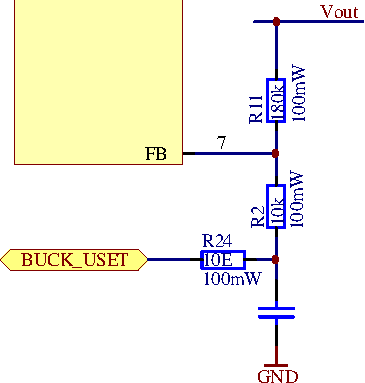
\includegraphics[width=.35\textwidth]{images/circuit/buck-uset.pdf}
    \caption{Einstellung der Ausgangsspannung durch \"Anderung der Bezugsspannung im Feedback-Loop mittels einer analogen Steuerspannung von 0V bis 1.21V}
    \label{fig:circuit:buck:uset}
\end{figure}

Analog zur Ausgangsspannung kann auch der Maximalstrom eingestellt werden. Durch
anlegen einer  analogen  Spannung  zwischen \SI{0}{\volt} und \SI{1.5}{\volt} am
Eingang  CTRL1 des LT3741 kann  direkt  der  maximale  \emph{Durchschnittsstrom}
durch die Spule $L_1$ und  somit  der maximale Ausgangsstrom eingestellt werden.

\begin{figure}[th!]
    \center
    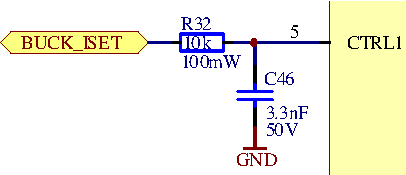
\includegraphics[width=.4\textwidth]{images/circuit/buck-iset.pdf}
    \caption{Einstellung des Maximalstroms mittels einer analogen Steuerspannung von 0V bis 1.5V}
    \label{fig:circuit:buck:iset}
\end{figure}

Die Abbildung \ref{fig:circuit:buck:iset} zeigt  die  dazugeh\"orige  Schaltung.
Der   maximale  durchschnittliche  Ausgangsstrom  $I_o$  wird  mit  der   Formel
\ref{eq:circuit:buck:output_current} berechnet

\begin{equation}
    I_o = \frac{U_{CTRL1}}{30 \cdot R_4}
    \label{eq:circuit:buck:output_current}
\end{equation}

wobei $U_{CTRL1}$ die  analoge  Steuerspannung vom zweiten DAC ist und $R_4$ der
\SI{10}{\milli\ohm}    Shunt-Widerstand    ist,   welcher   in   der   Abbildung
\ref{fig:circuit:buck} zu sehen ist.

Damit der Mikrocontroller angemessene Steuerspannungen  generieren kann, braucht
er die Ausgangsspannung und den Ausgangsstrom zu messen.

Die   Ausgangsspannung   wird   mittels   der   Schaltung   in   der   Abbildung
\ref{fig:circuit:buck:umeas} gemessen. Die Widerst\"ande $R_{12}$  und  $R_{15}$
wurden  so  dimensioniert  damit  die  Spannung  $BUCK\_UMEAS$  im  Bereich  von
\SI{0}{\volt} bis \SI{1.5}{\volt} skaliert ist.

\begin{figure}[th!]
    \center
    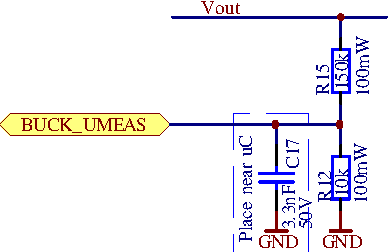
\includegraphics[width=.45\textwidth]{images/circuit/buck-umeas.pdf}
    \caption{Messen der Ausgangsspannung}
    \label{fig:circuit:buck:umeas}
\end{figure}

Der  Ausgangsstrom  wird  mittels  einem  Shunt-Widerstand  $R_5$  differentiell
gemessen.  Die  Schaltung dazu ist in der Abbildung \ref{fig:circuit:buck:imeas}
dargestellt.

\begin{figure}[th!]
    \center
    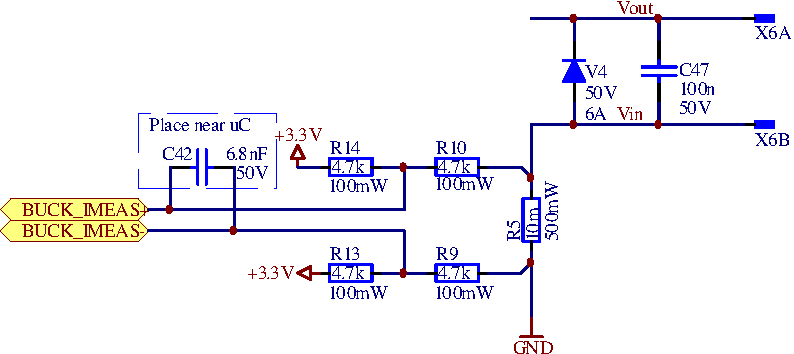
\includegraphics[width=.85\textwidth]{images/circuit/buck-imeas.pdf}
    \caption{Messen des Ausgangsstromes}
    \label{fig:circuit:buck:imeas}
\end{figure}

Es  ist  zu  beachten,  dass  die  Widerst\"ande  $R_{10}$  und  $R_{14}$  einen
Bias-Strom durch den Widerstand $R_5$  verursachen.  Somit  entsteht ein kleiner
Spannungs-Offset.
\begin{equation}
    U_{offset} = \frac{ \SI{3.3}{\volt} \cdot R_5 }{ R_{14} + R_{10} + R_5 }
    \label{eq:circuit:buck:shunt_offset}
\end{equation}

Da   der   ADC   eine   12-bit   Aufl\"osung   mit  einer  Referenzspannung  von
\SI{3.3}{\volt} hat, gilt:
\begin{equation}
    U_{step} = \frac{\SI{3.3}{\volt}}{2^{12}} = \SI{806}{\micro\volt}
    \label{eq:circuit:buck:adc_step}
\end{equation}

Die Widerst\"ande $R_9$, $R_{10}$, $R_{10}$ und  $R_{14}$  sollten  so klein wie
m\"oglich  dimensioniert  werden damit St\"orungen an  den  Leitungen  minimiert
werden  k\"onnen,  aber  sollten immer noch gross genug sein, damit  $U_{offset}
\leq  U_{step}$.  Zu  gross  d\"urfen  sie  auch  nicht  sein,  weil  sonst  die
Holding-Time  des   ADCs   nicht   mehr   erf\"ullt   ist  (was  bei  ca.  $\geq
\SI{5}{\kilo\ohm}$      der      Fall     ist).     Aus     den      Gleichungen
\ref{eq:circuit:buck:shunt_offset} und \ref{eq:circuit:buck:adc_step} kann jetzt
nach den 4 Widerst\"anden aufgel\"ost werden. Es gilt:
\begin{align*}
                          U_{step} &\geq U_{offset} \\
    \frac{\SI{3.3}{\volt}}{2^{12}} &\geq \SI{3.3}{\volt} \cdot \frac{R_5}{R_x + R_5} \\
                  \frac{1}{2^{12}} &\geq \frac{R_5}{R_x + R_5} \\
                               R_x &\geq \left( 2^{12} - 1 \right) \cdot R_5 \\
\end{align*}

wobei  $\frac{R_x}{2}  =  R_{9}  =  R_{10} = R_{13} = R_{14}$. Berechnet  ergibt
$\frac{R_x}{2} \approx \SI{22}{\ohm}$.

Eine weitere Einschr\"ankung, vorallem bei  kleinen  Widerst\"anden,  ist,  dass
nicht  unn\"otig  viel  Leistung  verbraten  werden sollte. Deshalb  werden  die
Widerst\"ande ein wenig h\"oher mit \SI{270}{\ohm} dimensioniert. In diesem Fall
ist der Leistungsverlust aller 4 Widerst\"ande:
\begin{equation*}
    P_{loss} \approx \frac{\SI{3.3}{\volt}^2}{2\cdot \SI{270}{\ohm}} \approx \SI{20}{\milli\watt}
\end{equation*}

Die gemessene Spannung  am  Shunt-Widerstand  ist recht klein. Deshalb verwenden
wir  den  im  Mikrocontroller  eingebauten  vorverst\"arker  (PGA),   was   eine
Verst\"arkung von bis  zu Faktor 64 erreichen kann. Das verst\"arkte Signal wird
intern an der eingebauten differentiellen ADC weitergeleitet.



% **************************************************************************** %
\subsubsection{Output}
% **************************************************************************** %

Two  banana  plugs  $X_{6A}$  and  $X_{6B}$  provide  the  connection  to  the
output  voltage,  while  reverse  voltage protection  is  achieved  via  diode
$V_4$.   (Figure \label{fig:circuit:output}).   An external  reference voltage
of  \SI{1.5}{\volt}  is  used to  ensure  that  the  ADCs  and DACs  can  make
accurate  measurements and  can  be used  over their  full  range (see  figure
\ref{fig:circuit:vref}).

\begin{minipage}{.50\textwidth}
    \center
    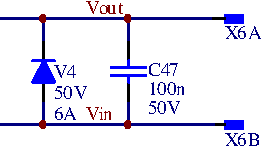
\includegraphics[width=.9\textwidth]{images/circuit/output-connectors.pdf}
    \captionof{figure}{Reverse voltage protection at output}
    \label{fig:circuit:output}
\end{minipage}
\begin{minipage}{.50\textwidth}
    \center
    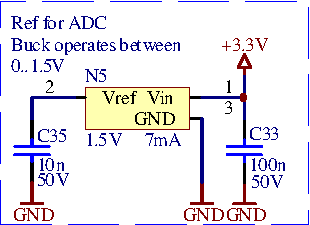
\includegraphics[width=.9\textwidth]{images/circuit/vref.pdf}
    \captionof{figure}{%
        \SI{1.5}{\volt} reference voltage for full-range operation of DACs
        and DACs
    }
    \label{fig:circuit:vref}
\end{minipage}



% **************************************************************************** %
\subsubsection{Enable and Under-Voltage Lockout circuit}
% **************************************************************************** %

The   LT3741's   \emph{Enable}   input   is   enabled   and   disabled   by  the
microcontroller's  $BUCK\_EN$ signal on one hand, on the other hand it is can be
forcibly  disabled  in  hardware  when  the  \SI{28}{\volt}  rail   drops  below
\SI{25}{\volt}. This  allows  for  a  controlled and predictable behavior of the
LT3741 during power-on  and power-off. The corresponding circuit can be found in
figure \ref{fig:circuit:uvlo}.

\begin{figure}[th!]
    \center
    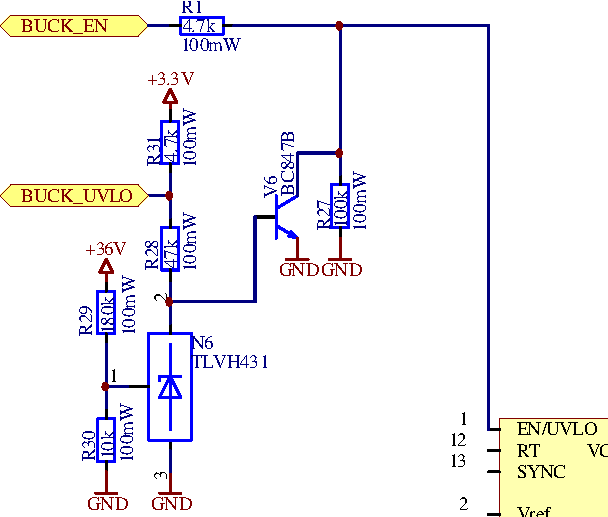
\includegraphics[width=.6\textwidth]{images/circuit/uvlo.pdf}
    \caption{Under-Voltage Lock-Out (UVLO) allows for controlled power-on and power-off of the controller}
    \label{fig:circuit:uvlo}
\end{figure}

In case of under-voltage, $N_6$ switches  on  and the transistor $V_6$ starts to
conduct,  thus  pulling  the  \emph{Enable}   input   to   \emph{Low}.   Voltage
$BUCK\_UVLO$ triggers an interrupt in the microcontroller.





% **************************************************************************** %
\subsection{Druck-Drehtaster}
% **************************************************************************** %

\begin{figure}[th!]
    \center
    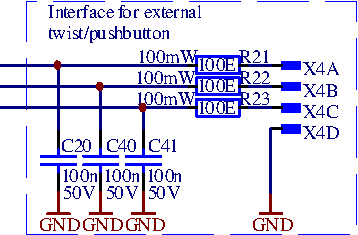
\includegraphics[width=.4\textwidth]{images/circuit/pushbutton.pdf}
    \caption{Drehdruckknopf}
    \label{fig:circuit:pushbutton}
\end{figure}





% **************************************************************************** %
\clearpage
\section{PCB}
\label{sec:pcb}
% **************************************************************************** %
When designing a PCB --  especially  when  a  switch-mode  power  converter is a
central  component  to  the  design  --  the  location  of  components and their
\emph{routing} (electrical connections) can be  critical  for correct operation.
Some  of  the  more  important  items  that  were  considered  are  listed here.
\begin{itemize}
    \item
        High frequency, high power loops are routed as tightly as possible.
    \item
        Sensitive, high impedance traces are kept separate from other signals
        and routed as differential pairs where necessary.
    \item
        Digital logic is kept separate from analog and high power circuitry.
    \item
        Power rails and their bypass capacitors need to be placed intelligently.
    \item
        Larger copper areas can be used to meet heat dissipation requirements.
    \item
        The positioning of mechanical parts can be annoying because they take up
        way more space than what one might initially, naively, expect.
\end{itemize}

\begin{minipage}{0.5\textwidth}
    Figure \ref{fig:pcb:partitioning}  shows how  our \SI{60x60}{\milli\meter}
    printed  circuit  board  is  partitioned.  In  particular  we  would  like
    to  emphasise   how  the  ground  plane   has  been  split  from   top  to
    bottom,  physically separating  partition  \emph{A} from  the other  three
    partitions,  and how  the LT3741  is placed  in the  center where  the two
    planes  join.   Partition  \emph{A}  contains  high  power/high  frequency
    components,  such as  the two  switching  MOSFETs, the  inductor, and  the
    output  capacitors, whereas  the other  partitions contain  more sensitive
    circuitry (in particular partition \emph{C}). The split helps minimize any
    crosstalk. The LT3741  chip is placed at  the joining position of  the two
    split planes because  it must communicated with the digital  logic as well
    as power the high power circuitry.

    Partition \emph{C}  contains the micro controller,  LCD header, push/twist
    button header and other digital components.

\end{minipage}
\begin{minipage}{0.5\textwidth}
    \centering
    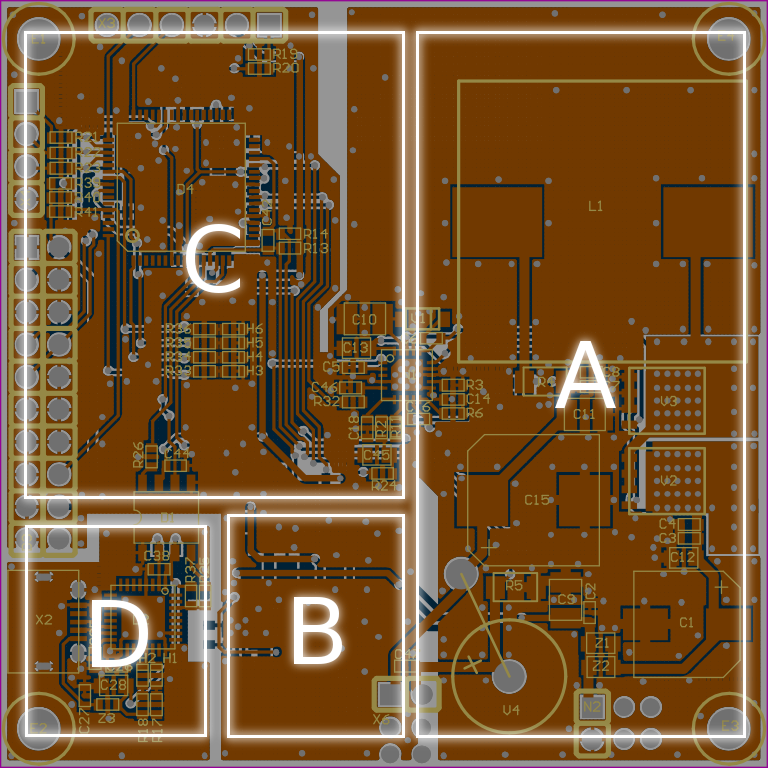
\includegraphics[width=.9\linewidth]{images/pcb/partitioning.png}
    \captionof{figure}{Partitioning scheme of component groups.
        \textbf{A:} High power components
        \textbf{B:} Voltage rails
        \textbf{C:} Digital logic
        \textbf{D:} Isolated transceiver logic
    }
    \label{fig:pcb:partitioning}
\end{minipage}

    Partition \emph{B} contains the  components responsible for generating the
    three voltage  rails discussed in section  \ref{sec:voltage_rails}. It was
    placed at  the bottom of  the board where the  power input is  located, to
    minimize the trace  lengths required for power distribution  on the board,
    and  it  was also  placed  far  away  from  partition \emph{B}  such  that
    interference with the digital circuitry is minimized.

    Partition \emph{D} is  electrically isolated from the rest  of the circuit
    and contains  the components  responsible for  USB communication.   It was
    isolated because  the voltage potential of  a connected USB device  may be
    different than the potential our device is running on.

    It  is  critical for  the  total  physical length  of  these  loops to  be
    minimized. Our solution can  be seen in the physical PCB  layout in figure
    \ref{fig:pcb:loops2}.

\begin{minipage}{0.5\textwidth}
    Figure  \ref{fig:pcb:loops1}  shows the  two  critical  loops where  short
    intervals  of high  amounts  of  current flow  in  this design. The  first
    (green) loop is  active when the switching MOSFET $V_2$  is conducting and
    transferring  charge  from  the  input  bypass  capacitors  $C_3$,  $C_4$,
    $C_{12}$ and $C_1$ through the resistor $R4$ into the inductor $L_1$.  The
    second (blue) loop is active when the switching mosfet $V_3$ is conducting
    and transferring charge from the inductor $L_1$ through the resistor $R_4$
    into the output bypass capacitors $C_{15}$, $C_{11}$, $C_7$ and $C_8$.

\end{minipage}
\begin{minipage}{0.5\textwidth}
    \centering
    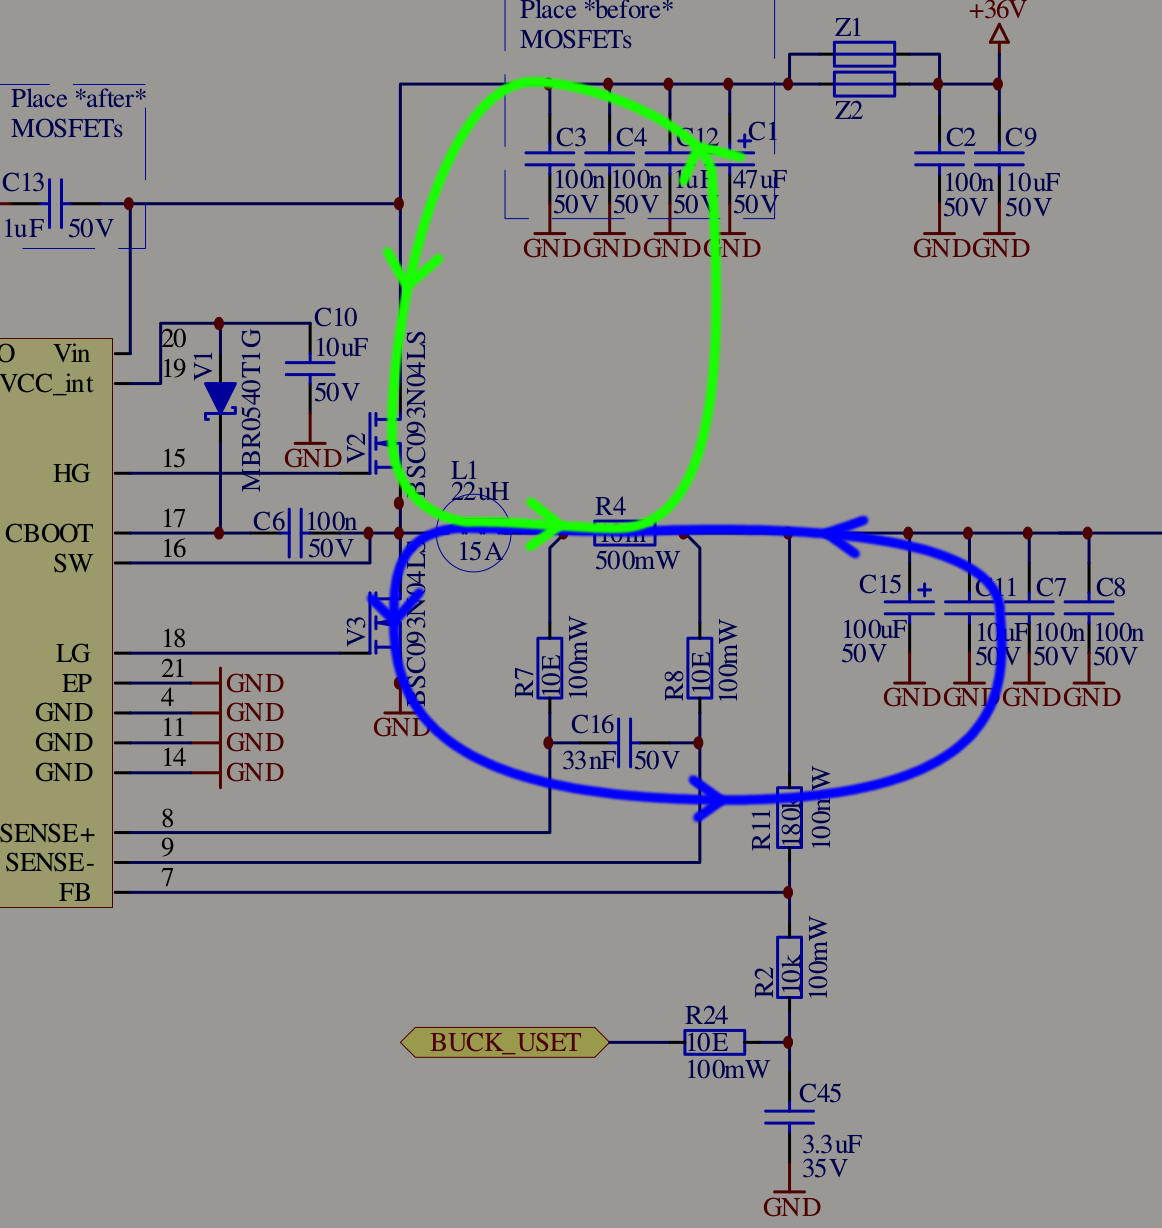
\includegraphics[width=\textwidth,trim=0 25mm 0 0,clip]{images/circuit/schematic_high_current.png}
    \captionof{figure}{Critical high current, high frequency loops in the schematic. Blue indicates the current path of the first critical loop, green the second.}
    \label{fig:pcb:loops1}
\end{minipage}

\begin{figure}[h!]
    \center
    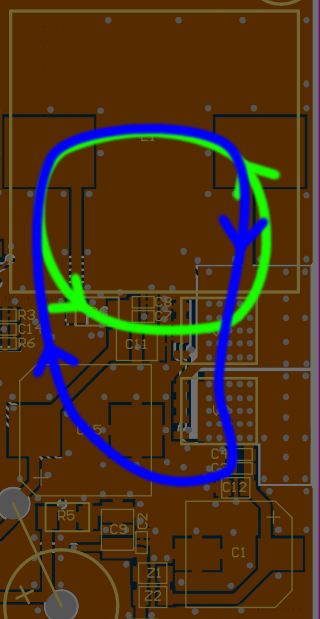
\includegraphics[width=.3\textwidth]{images/pcb/buck2.png}
    \caption{High current, high frequency loops are routed as tightly as possible}
    \label{fig:pcb:loops2}
\end{figure}



% **************************************************************************** %
\clearpage
\section{Software}
\label{sec:software}
% **************************************************************************** %
Dokumentation Software



% **************************************************************************** %
\clearpage
\section{Verifikation}
\label{sec:verification}
% **************************************************************************** %
\begin{itemize}
    \item
        U und I bei verschiene Lasten, siehe Pflichtenheft.
            ==> Kurven plotten (gemessen und berechnet).
    \item
        Transienten, Laständerungen
    \item
        Leistungsaufnahme
    \item
        Dings funktioniert nicht
    \item
        Structure:
            1) Definition of test fixture
            2) What we actually did
            3) Error analysis
\end{itemize}


\subsection{Definition of test fixture}





% **************************************************************************** %
\clearpage
\section{Fazit}
\label{sec:conclusion}
% **************************************************************************** %
Conclusion: Lots and lots of work.



% **************************************************************************** %
%\clearpage
%\section*{Unterschrift}
%\label{sec:signature}
% **************************************************************************** %
%\input{sections/signature.tex}


% **************************************************************************** %
%\clearpage
%\begin{appendices}
%    %\appendixpage
%    %\addappheadtotoc
%    %\appendix
%    %\section{Anhang}
%    \label{sec:appendix}
%    % ************************************************************************ %
%    % **************************************************************************** %
\clearpage
\section{Specifications}
\label{appendix:specs}
% **************************************************************************** %

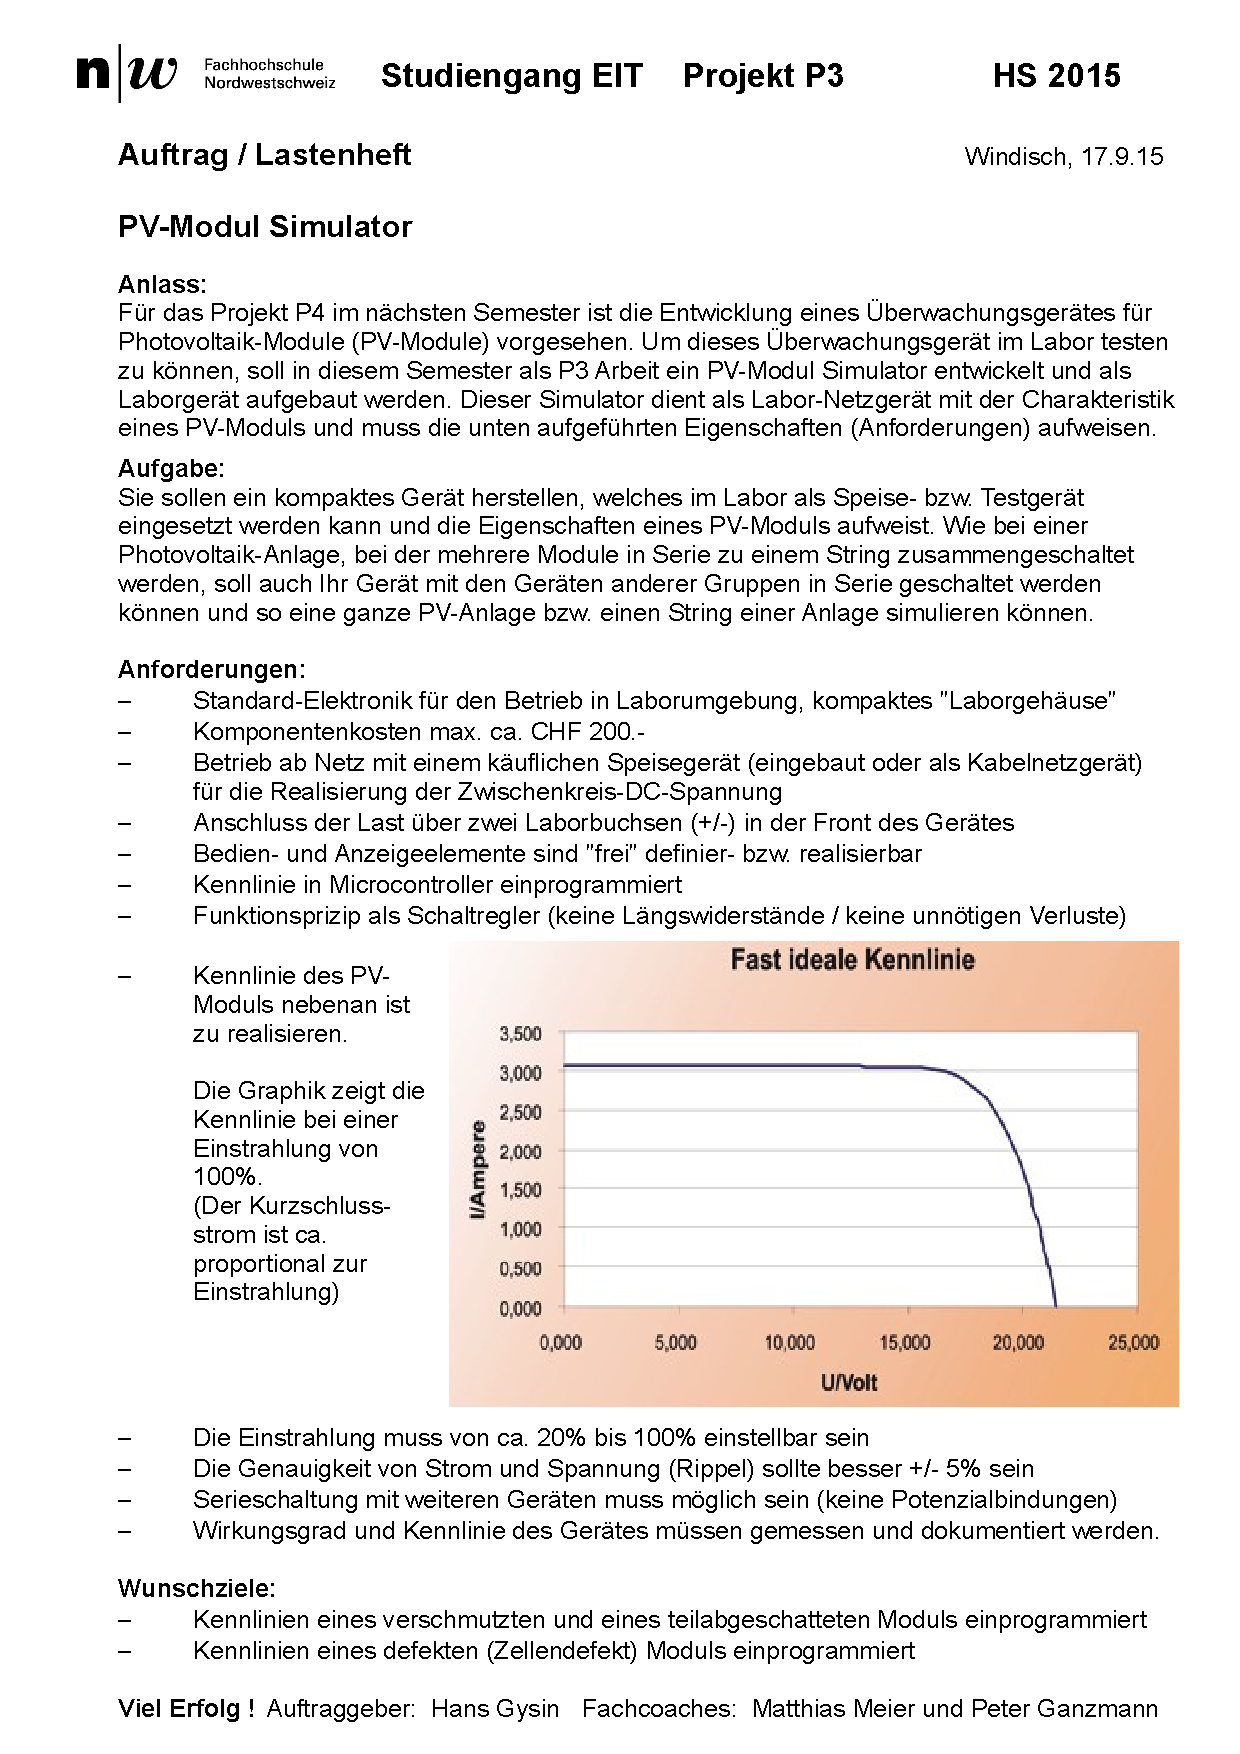
\includepdf[pages=-,scale=1]{images/specs.pdf}
%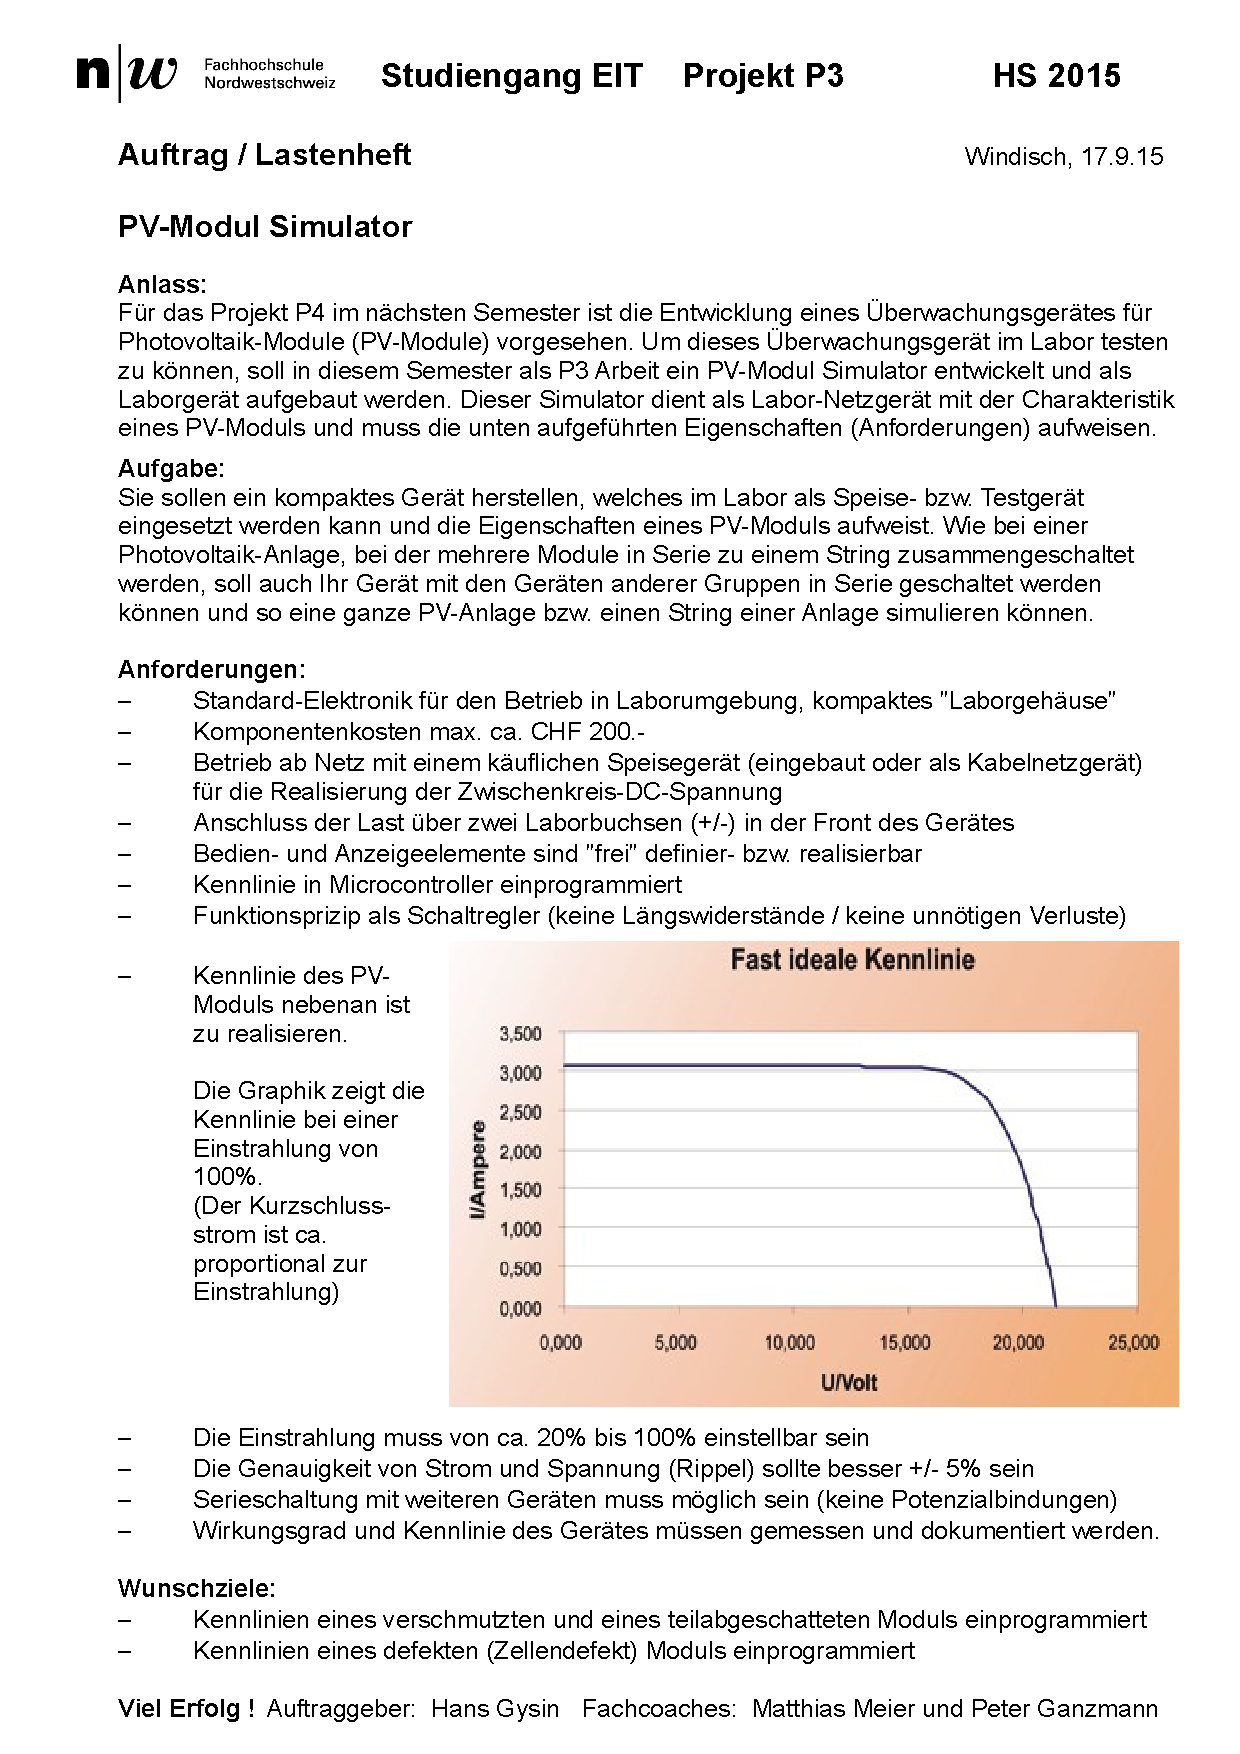
\includegraphics[width=\paperwidth]{images/specs.pdf}

{%START A3 PAGES
    \clearpage
    \pdfpagewidth=2\pdfpagewidth
    \textwidth=2\textwidth
    \addtolength{\textwidth}{50mm}

    % **************************************************************************** %
    \section{LT3471 Circuit}
    \label{appendix:lt3741:circuit}
    % **************************************************************************** %

    \begin{minipage}[b]{.5\textwidth}
        The   circuit    used   to    control   the   LT3471    is   described
        in   detail   in   section  \ref{subsec:lt3741}   starting   on   page
        \pageref{subsec:lt3741}. For the  reader's convenience,  the schematic
        in Figure \ref{fig:circuit:buck} is intended to be folded out and kept
        open as  a reference while  reading that section of  this report. This
        allows  for  convenient  cross-checking  between  text  and  schematic
        without needing  to constantly  scroll through  the report's  pages or
        needing to insert multiple copies of Figure \label{fig:circuit:buck}.
    \end{minipage}%
    \begin{minipage}[b]{.5\textwidth}
        \center
        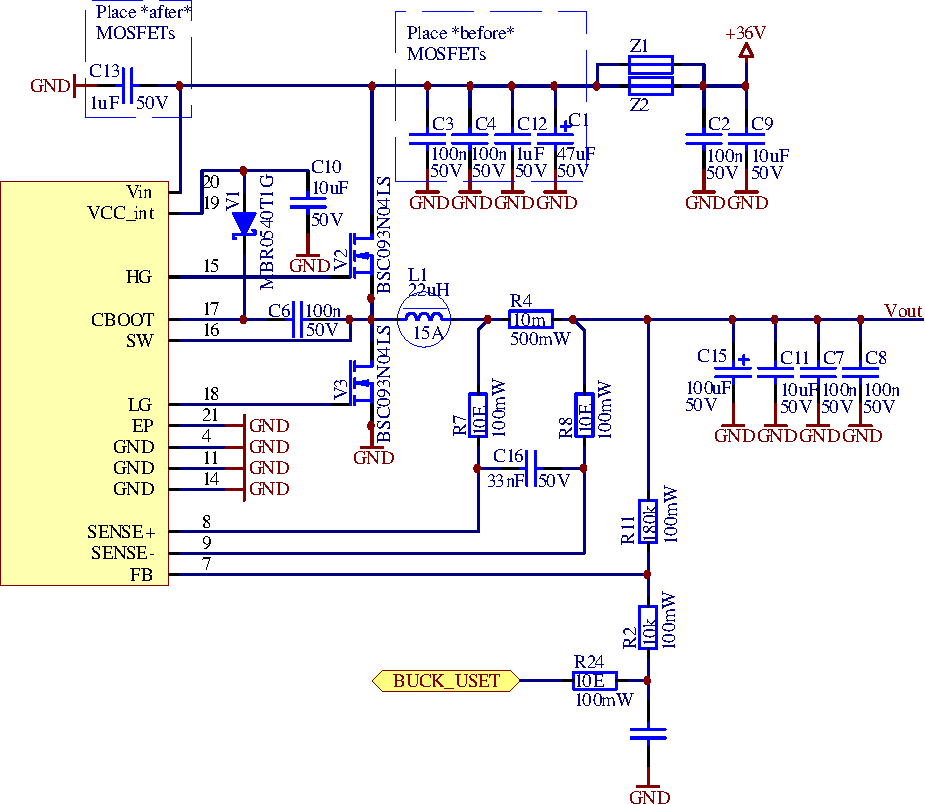
\includegraphics[width=.67\textwidth]{images/circuit/buck.pdf}
        %\caption{Herzst\"uck des Projektes: Aufbau des LT3741 CVCC Synchronwandler}
        \captionof{figure}{The device's heart: Overview over circuit for the LT3741 CCVC synchronous converter.}
        \label{fig:circuit:buck}
    \end{minipage}

\clearpage
}

\setlength\paperheight{297mm}
\setlength\paperwidth{420mm}
\setlength\pdfpageheight{\paperheight}
\setlength\pdfpagewidth{\paperwidth}

    % **************************************************************************** %
    \section{List of Components}
    \label{appendix:components}
    % **************************************************************************** %
    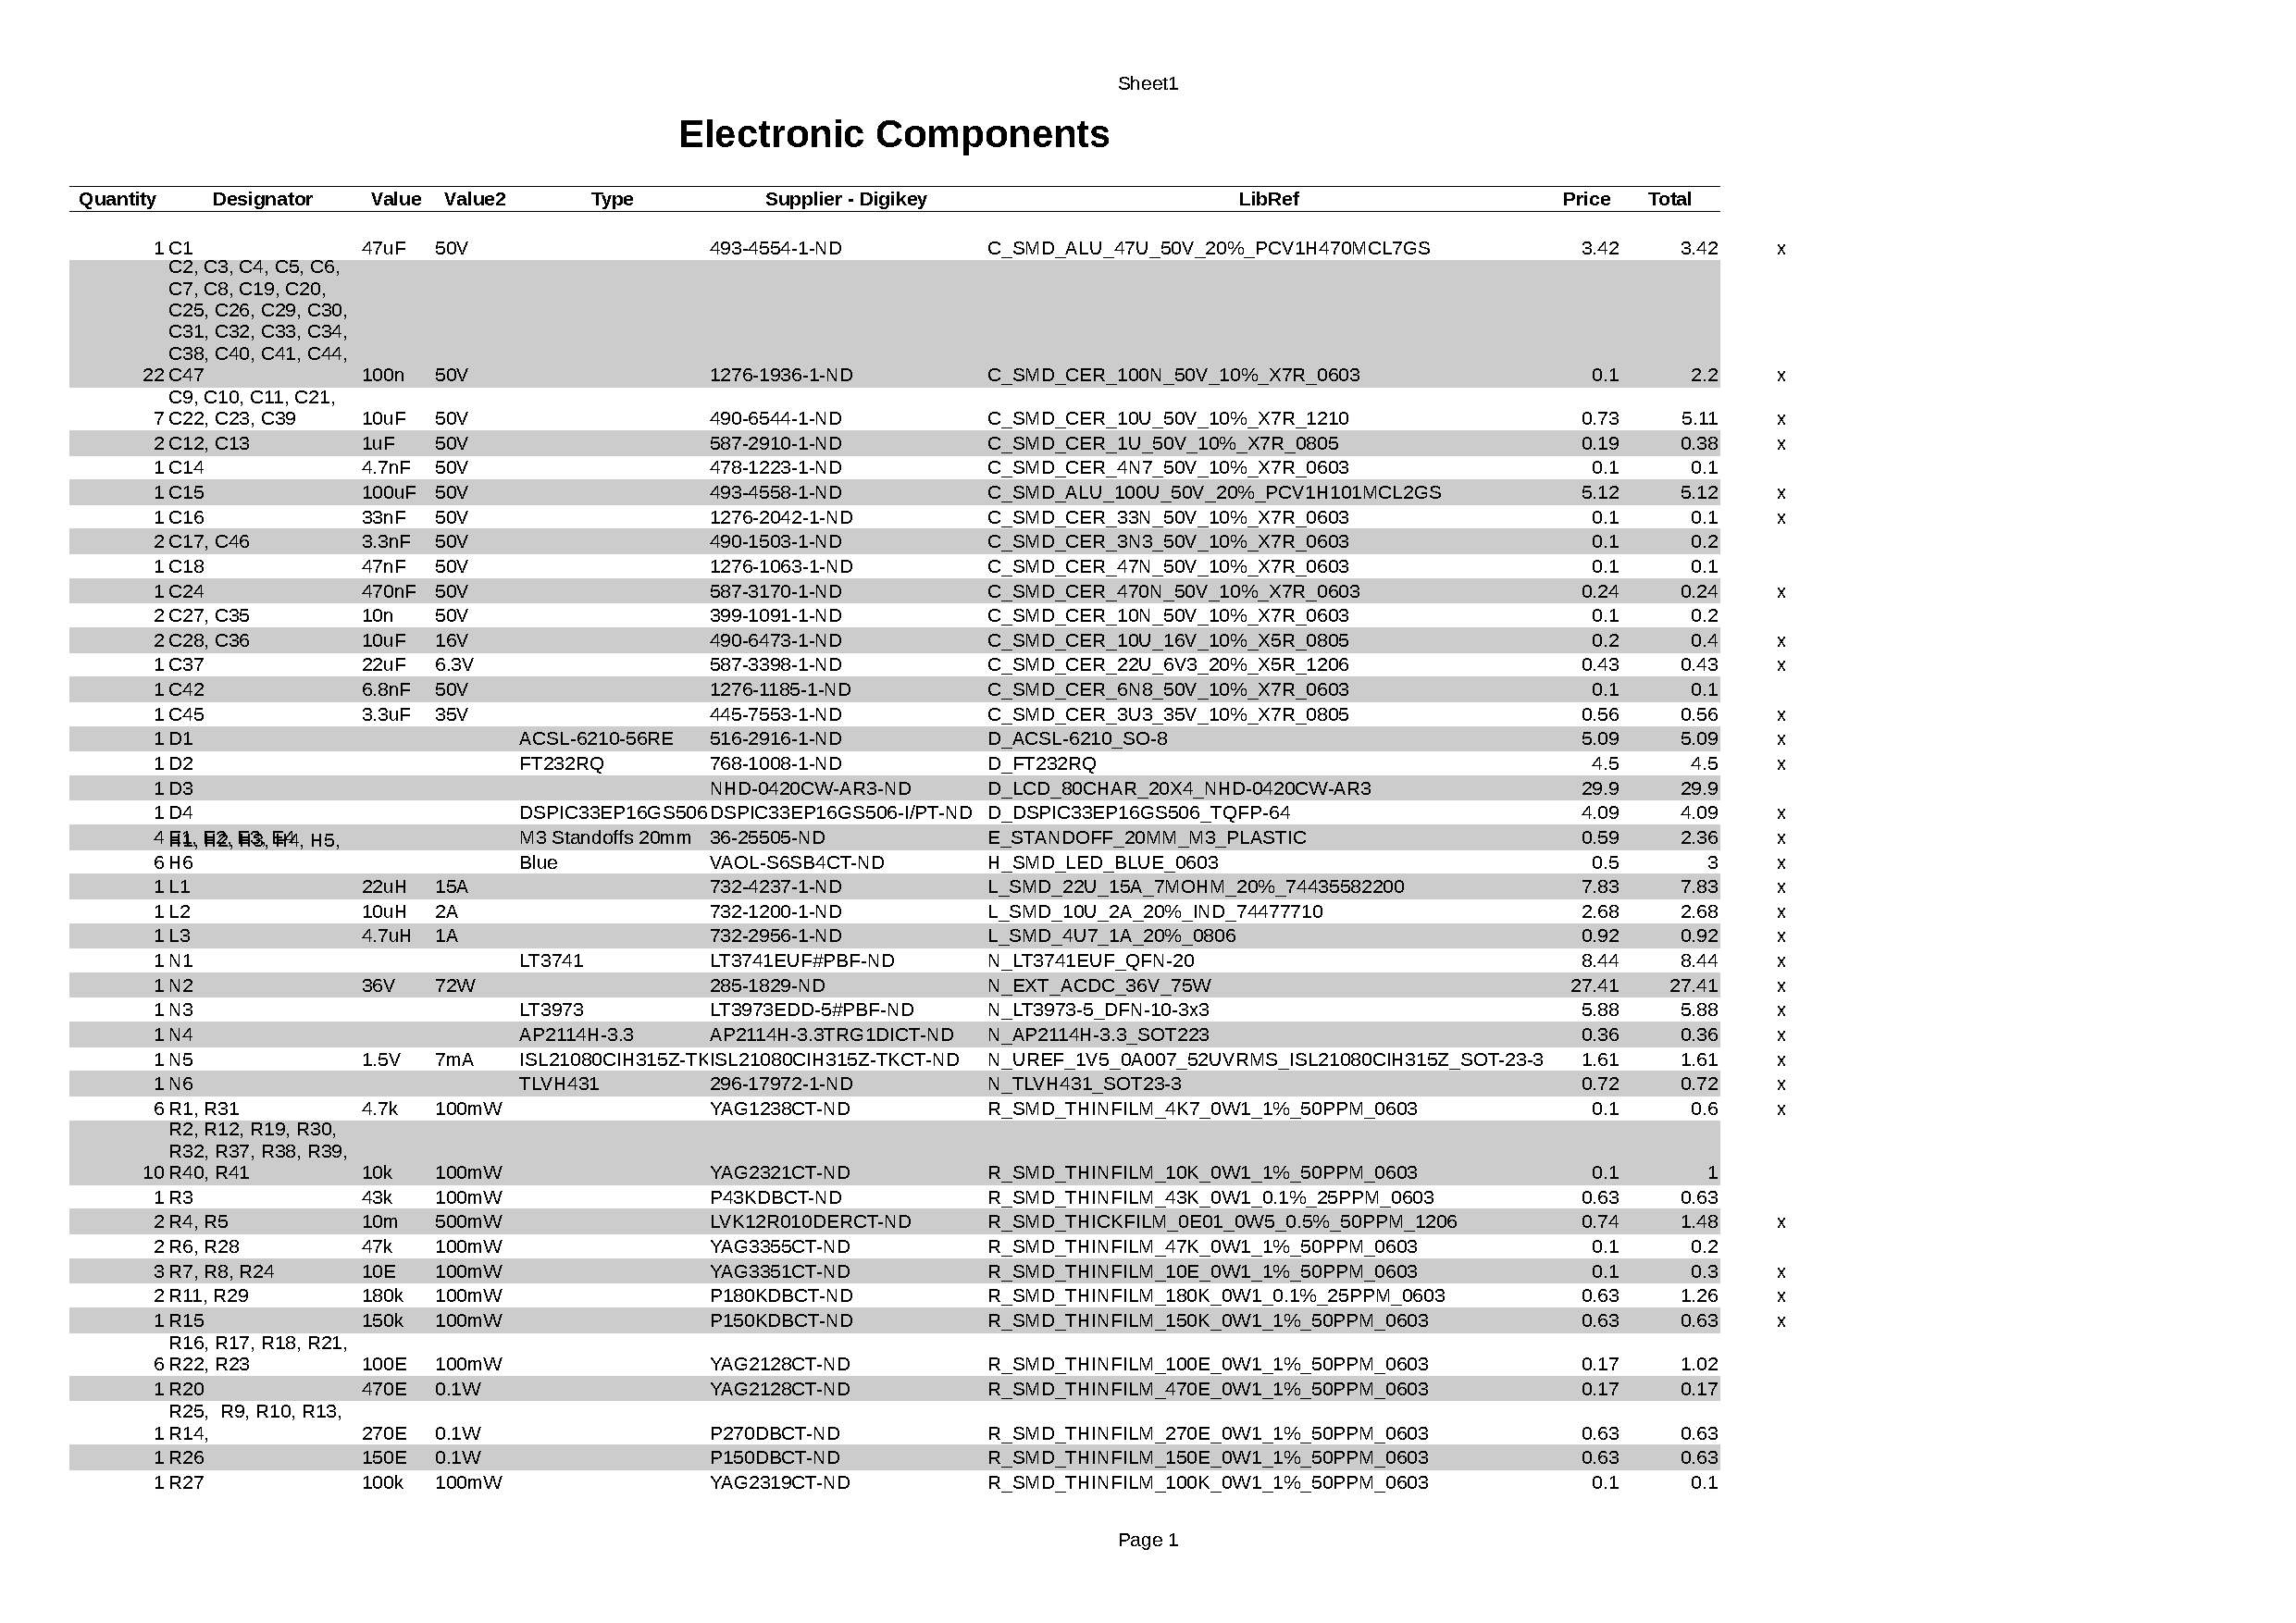
\includepdf[pages=-,scale=1]{images/bom.pdf}

\setlength\paperheight{210mm}
\setlength\paperwidth{297mm}
\setlength\pdfpageheight{\paperheight}
\setlength\pdfpagewidth{\paperwidth}




% **************************************************************************** %
\clearpage
\section{Inductors}
\label{appendix:inductors}
% **************************************************************************** %

Filtering available  inductors according to  the criteria outlined  in section
\ref{subsubsec:lt3741:inductors} on  page \pageref{subsubsec:lt3741:inductors}
left us  with the models listed  in Table \ref{tab:circuit:buck:inductor}. The
model highlighted  in grey  was selected  due to it  having the  lowest direct
current resistance (DCR).

\begin{table}[th!]
    \begin{center}
        \caption{List of inductors matching our requirements}
        \label{tab:circuit:buck:inductor}
        \begin{tabular}{lcccc}
            \toprule
            Digikey         & Price (CHF) & Inductance (\SI{}{\micro\henry}) & DCR (\SI{}{\ohm}) & Ohmic Loss (\SI{}{\watt}) \\
            \midrule
            \rowcolor{lightgray}
            732-4237-1-ND   & 8.03        & 22                               & 0.007             & 0.175  \\
            732-2179-1-ND   & 6.4         & 47                               & 0.0335            & 0.8375 \\
            732-2177-1-ND   & 6.4         & 22                               & 0.0146            & 0.365  \\
            \bottomrule
        \end{tabular}
    \end{center}
\end{table}


% **************************************************************************** %
\section{MOSFETs}
\label{appendix:mosfets}
% **************************************************************************** %

Table     \ref{tab:circuit:buck:mosfet}     lists    MOSFETs     that     meet
the    constraints     outlined    in     \ref{subsubsec:lt3741:mosfets}    on
\pageref{subsubsec:lt3741:mosfets}.  For each one  the power losses $P_{LOSS}$
and $P_{LOSS\_LDO}$ were calculated.

\begin{table}[th!]
    \begin{center}
        \caption{Possible choices for MOSFETs}
        \label{tab:circuit:buck:mosfet}
        \begin{tabular}{cccccccccc}
            \toprule
            $R_{DS_{(on)}}$ & $Q_{GD}$ & $Q_{GS}$ & $R_G$ & $V_{GS_{THR}}$ & Ohmic Loss & Transision Loss & Total Loss & Drive Loss \\
            \midrule
            0.0032          & 4        & 2.5      & 0.4   & 2.5            & 0.104      & 1.0296          & 1.1336     & 0.806 \\
            0.0039          & 7        & 9        & 2.4   & 3.3            & 0.12675    & 4.8384          & 4.96515    & 1.984 \\
            0.0042          & 7        & 9        & 2.4   & 3.3            & 0.1365     & 4.8384          & 4.9749     & 1.984 \\
            0.008           & 2        & 4.5      & 3     & 2              & 0.26       & 2.2464          & 2.5064     & 0.558 \\
            0.0067          & 5.3      & 3.9      & 1.5   & 1              & 0.21775    & 2.18592         & 2.40367    & 0.7998 \\
            \rowcolor{lightgray}
            0.0093          & 2        & 4.9      & 1     & 2              & 0.30225    & 1.39104         & 1.69329    & 1.488 \\
            0.019           & 8        & 4        & 1.3   & 2              & 0.6175     & 2.6784          & 3.2959     & 1.798 \\
            0.0095          & 7.5      & 6        & 1     & 3              & 0.30875    & 2.7216          & 3.03035    & 1.736 \\
            \bottomrule
        \end{tabular}
    \end{center}
\end{table}


The MOSFET highlighted in grey was selected.  Though it is not the best model,
it is a lot  cheaper than the best fit and  has better documentation. The same
MOSFET is used for both the low-side and the high-side switch.


%\end{appendices}

% **************************************************************************** %
%\clearpage
%\phantomsection
%\addcontentsline{toc}{section}{\bibname}
%\bibliography{bibliography/bibliography}{\bibliographystyle{bibliography/deIEEEtran.bst}}
% **************************************************************************** %
\end{document}
